\clearpage
\Question{Union-find}

\begin{minipage}[t]{0.55\linewidth}
Consider the 7-vertex weighted graph with 12 edges shown to the right
of this text.
\end{minipage}%
\hfill
\begin{minipage}[t]{0.45\linewidth}
\hfill
\raisebox{-25ex}[0ex][25ex]{%
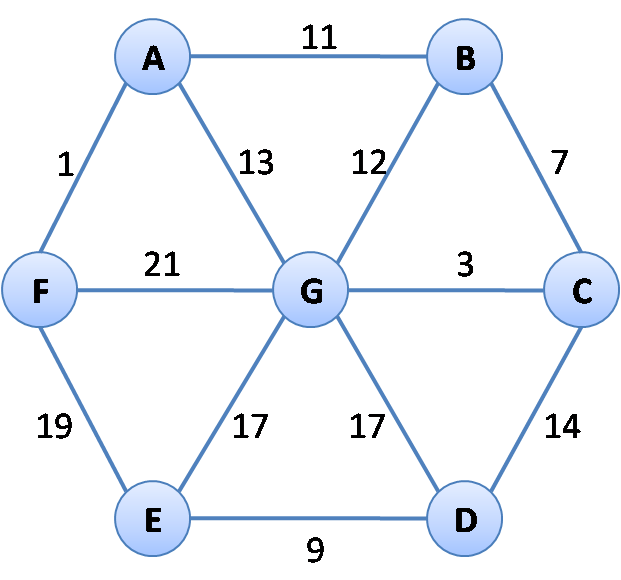
\includegraphics[width=0.87\linewidth]{\img/wheel6.png}}
\end{minipage}

\begin{parts}
\ifbool{practice}{\part}{\bonuspart[1]}%
\TAGS{union-find}%
We will compute a minimum spanning tree for this graph using the
union-find algorithm with \emph{height tracking}.  To this end,
complete the following table.  Each row corresponds to the contents of
the union-find data structure after considering one of the edges in
this graph \emph{(there are enough rows to compute a minimum spanning
  tree, but possibly more rows than you need}).

When merging trees, if you have a choice as to which vertex to make
the canonical representative, pick the one that comes alphabetically
last: for example, when adding edge $AB$, if $A$ has canonical
representative $G$ and $B$ has canonical representative $D$ \emph{and
  either $G$ or $D$ could be chosen as the new canonical
  representative}, we ask that you pick $G$.

\begin{center}
\newcommand{\vname}[1]{\multicolumn{1}{c}{\textbf{#1}}}
\newcommand{\vnum}[1]{\multicolumn{1}{r}{\raisebox{-0.5ex}{\footnotesize #1}}}
\newcommand{\adding}[1]{Considering edge \uanswer{4em}{#1}}
\newcommand{\SP}[1]{\answer{2.25em}{#1}}
\newcommand{\BP}[1]{\SP{\textbf{#1}}}
\renewcommand{\arraystretch}{1.5}
\begin{tabular}{@{}l|*{7}{c|}}
   \multicolumn{1}{@{}r}{\textbf{\em Vertex name}}
 & \vname{A} & \vname{B} & \vname{C} & \vname{D} & \vname{E} & \vname{F} & \vname{G}
\\ \multicolumn{1}{@{}r}{\small\raisebox{-0.5ex}{\em Vertex number}}
 & \vnum{0} & \vnum{1} & \vnum{2} & \vnum{3} & \vnum{4} & \vnum{5} & \vnum{6}
\\\cline{2-8}
Initially
 & -1    & -1 & -1 & -1 & -1 & -1 & -1
\\\cline{2-8}
\adding{AF}
 & \BP{5}&\SP{-1}&\SP{-1}&\SP{-1}&\SP{-1}&\BP{-2}&\SP{-1}
\\\cline{2-8}
\adding{CG}
 & \SP{5}&\SP{-1}&\BP{6} &\SP{-1}&\SP{-1}&\SP{-2}&\BP{-2}
\\\cline{2-8}
\adding{BC}
 & \SP{5}&\BP{6} &\SP{6} &\SP{-1}&\SP{-1}&\SP{-2}&\SP{-2}
\\\cline{2-8}
\adding{DE}
 & \SP{5}&\SP{6} &\SP{6} &\BP{4} &\BP{-2}&\SP{-2}&\SP{-1}
\\\cline{2-8}
\adding{AB}
 & \SP{5}&\SP{6} &\SP{6} &\SP{4} &\SP{-2}&\BP{6} &\BP{-3}
\\\cline{2-8}
\adding{BG}
 & \SP{5}&\SP{6} &\SP{6} &\SP{4} &\SP{-2}&\SP{6} &\SP{-3}
\\\cline{2-8}
\adding{AG}
 & \SP{5}&\SP{6} &\SP{6} &\SP{4} &\SP{-2}&\SP{6} &\SP{-3}
\\\cline{2-8}
\adding{CD}
 & \SP{5}&\SP{6} &\SP{6} &\SP{4} &\BP{6} &\SP{6} &\SP{-3}
\\\cline{2-8}
\adding{}
 & \SP{}&\SP{}&\SP{}&\SP{}&\SP{}&\SP{}&\SP{}
\\\cline{2-8}
\adding{}
 & \SP{}&\SP{}&\SP{}&\SP{}&\SP{}&\SP{}&\SP{}
\\\cline{2-8}
\end{tabular}
\end{center}

\RUBRIC
Part (a)
TAGS: union-find

Gradescope rubric:
+0.25pt  considers edges in order (AF, CG, BC, DE, AB, BG, AG, CD ...)
+0.5pt   first 5 correct
+0.25pt  last 3 correct
-0.1pt   edges BG and AG omitted
-0.1pt   went past early termination

Commentary:
- edge order: AF, CG, BC, DE, AB, BG, AG, CD ... EG or DG, EF, FG)


Vertex Name
Vertex number         0   1   2   3   4   5   6
Initially            -1  -1  -1  -1  -1  -1  -1
Considering __AF__   _5_ -1  -1  -1  -1 _-2_ -1
Considering __CG__    5  -1  _6_ -1  -1  -2 _-2_
Considering __BC__    5  _6_  6  -1  -1  -2  -2
Considering __DE__    5   6   6  _4__-2_ -2  -2
Considering __AB__    5   6   6   4  -2  _6__-3_
Considering __BG__    5   6   6   4  -2   6  -3  (unchanged)
Considering __AG__    5   6   6   4  -2   6  -3  (unchanged)
Considering __CD__    5   6   6   4  _6_  6  -3
  (other lines are not needed)
ENDRUBRIC

\newpage
\ifbool{practice}{\part}{\bonuspart[1]}%
\TAGS{union-find}%
Using the template below, draw the spanning tree obtained through the
calculation in the last task, and give the graphical representation
of the final state of the union-find data structure.

\begin{framed}
\begin{tabular}{c@{}@{}}
   \textbf{Spanning tree}
\\\\[1ex]
   \ifprintanswers
     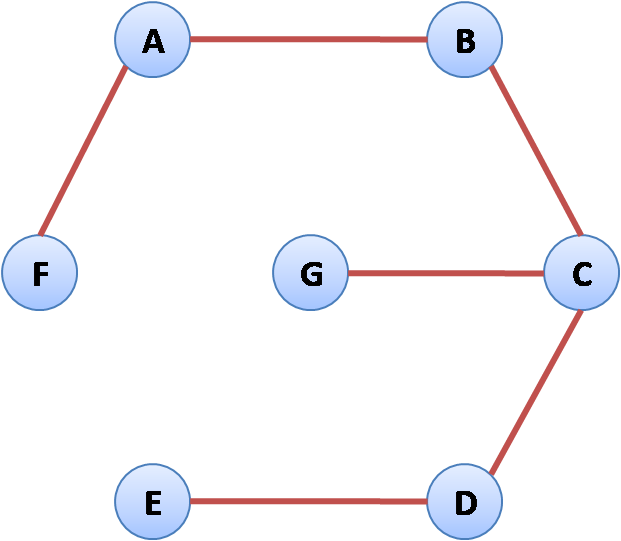
\includegraphics[width=0.45\linewidth]{\img/wheel6-spanning.png}
   \else
     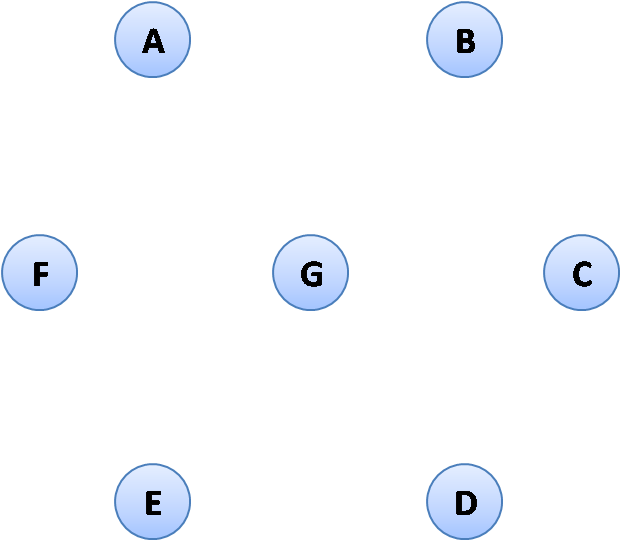
\includegraphics[width=0.45\linewidth]{\img/wheel6-empty.png}
   \fi
\end{tabular}
\hfill\rule[-18ex]{0.01em}{36ex}\hfill
\begin{tabular}{@{}c@{}}
   \textbf{Union-find graph}
\\\\[1ex]
   \ifprintanswers
     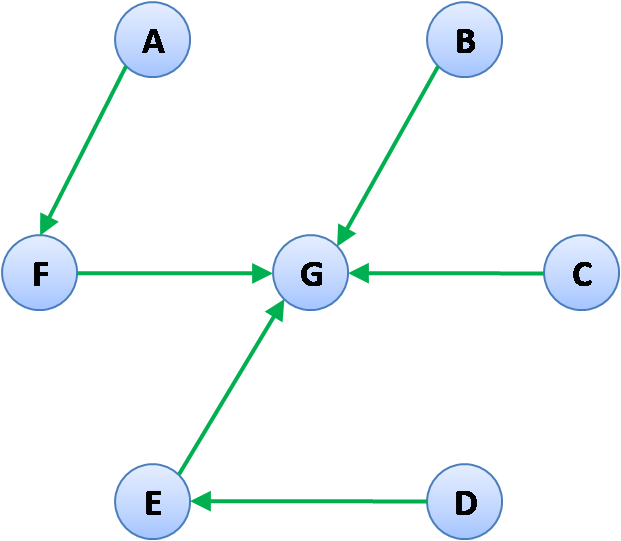
\includegraphics[width=0.45\linewidth]{\img/wheel6-ht.png}
   \else
     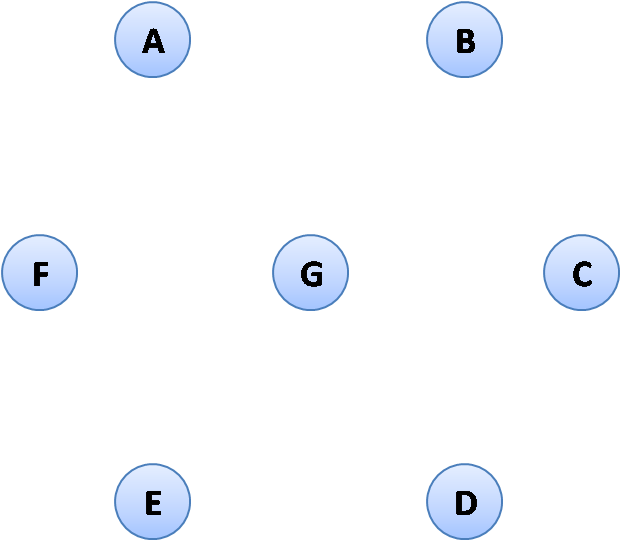
\includegraphics[width=0.45\linewidth]{\img/wheel6-empty.png}
   \fi
\end{tabular}
\end{framed}

\RUBRIC
Part (b)
TAGS: union-find

Gradescope rubric:
+0.25pt  Correct spanning tree (AF, AB, BC, CD, DE, CG)
+0.25pt  Correct UF graph (AF, FG, EG, DE, CG, BG)

Commentary: (none)
ENDRUBRIC

\ifbool{practice}{\part}{\bonuspart[1]}%
\TAGS{union-find}%
Starting from the original weighted graph for this question, draw the
graphical representation of final state of the union-find data
structure assuming that we used the variant of the union-find
algorithm that uses both height tracking \emph{and path compression}.


\begin{framed}
\begin{center}
\begin{tabular}{c}
   \textbf{Union-find graph with path compression}
\\\\[1ex]
   \ifprintanswers
     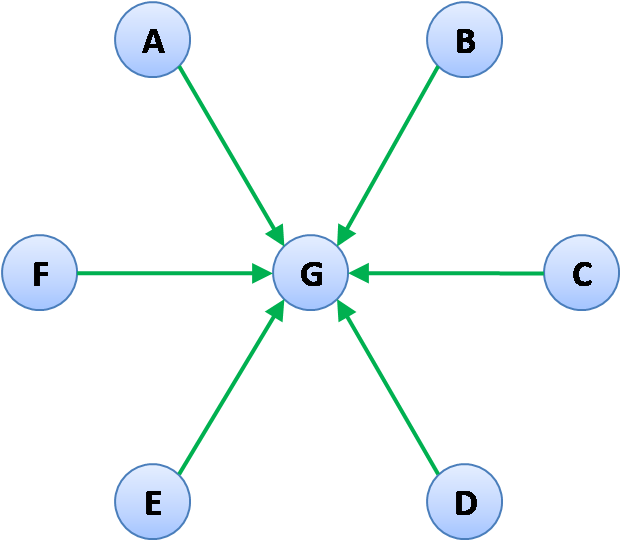
\includegraphics[width=0.45\linewidth]{\img/wheel6-pc.png}
   \else
     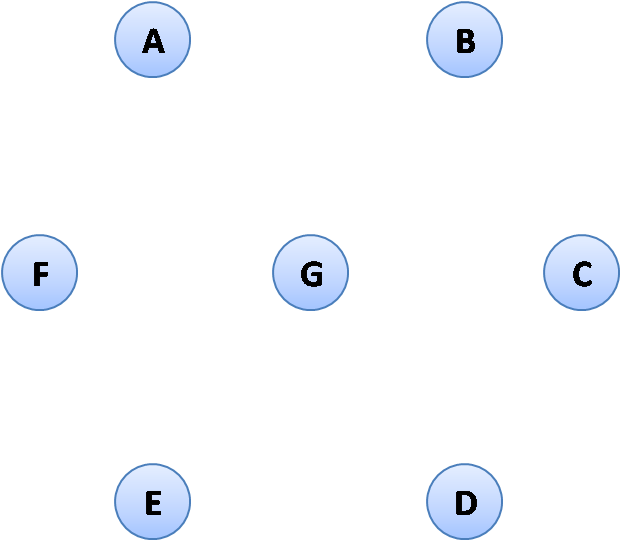
\includegraphics[width=0.5\linewidth]{\img/wheel6-empty.png}
   \fi
\end{tabular}
\end{center}
\end{framed}


\RUBRIC
Part (c)
TAGS: union-find

Gradescope rubric:
+0.25pt  Correct UF graph (AG, BG, CG, DG, EG, FG)

Commentary: (none)
ENDRUBRIC

\end{parts}
